%!TEX root = ../thesis.tex

\chapter{Реалізація спрощеної версії гібридної криптографічної схеми Kyber}
\label{chap:chapter1}  

У цьому розділі розглянуто реалізацію спрощеної версії гібридної криптографічної схеми Kyber~\cite{KyberWebsite}. Для цього спочатку буде проведено короткий огляд загальної схеми КЕМ Kyber, яка є постквантовою криптосистемою стійкість якої ґрунтується на складності розв’язання задачі навчання на помилках (LWE) над модульними решітками. Далі буде розглянуто Baby Kyber – спрощену версію схеми, яка дозволяє проаналізувати основні принципи роботи Kyber у спрощеному вигляді~\cite{babyKyber}. Теоретичне обґрунтування Baby Kyber допоможе зрозуміти його основні компоненти та алгоритми. Нарешті, буде представлена практична реалізація Baby Kyber, включаючи опис використаних криптографічних примітивів, алгоритми обміну ключами та результати тестування.

%%% --------------------------------------------------------
\section{Огляд криптосистеми Kyber}
%%% -------------------------------------------------------- 

Kyber – це постквантова криптографічна схема для обміну ключами, що ґрунтується на задачах решіткової криптографії. Вона була розроблена для забезпечення стійкості до атак квантових комп’ютерів і стала одним із фіналістів конкурсу NIST з постквантової криптографії.  

У цьому підрозділі буде розглянуто загальну схему роботи Kyber, включаючи основні алгоритми генерації ключів, шифрування та розшифрування. Також буде проаналізовано властивості та рівень безпеки Kyber, зокрема її стійкість до криптографічних атак і ефективність у практичному застосуванні.

\subsection*{Загальна схема роботи Kyber}

Kyber є пост-квантовим КЕМ, що використовує відкритий ключ. Ця схема є першою схемою КЕМ, який стандартизовано.  Механізм інкапсуляції ключів Kyber використовує задачу модульного навчання на помилках (MLWE)~\cite{Langlois2012} та складність її розв'язання. Тобто Kyber - це захищений IND-CCA механізм інкапсуляції ключів (KEM), стійкість якого ґрунтується на складності розв'язання задачі навчання на помилках (LWE) над модульними решітками~\cite{KyberWebsite}.  Звичайно, існують аналогічні схеми, які ґрунтуються на неструктурованому MLWЕ, проте ця конструкція має значно більші переваги в ефективності~\cite{Gonzalez2021}.

Для побудови Kyber спершу вводиться IND-CPA-безпечна схема шифрування з відкритим ключем, яка використовується для шифрування повідомлення фіксованої довжини, після цього, використовуючи FO-перетворення, будується IND-CCA2-безпечний КЕМ~\cite{KyberWebsite}.

Структура Kyber ґрунтується на модульній версії схеми шифрування Ring-LWE LPR~\cite{Lyubashevsky2013, Langlois2012} із відкиданням бітів~\cite{Pessl2017}. Цей КЕМ також посилений багатьма поліпшеними реалізаціями схем шифрування на основі решітки, таких як NewHope~\cite{Alkim2016}. У схемах шифрування, що використовуються (NewHope та схемах Ring-LWE) операції мали вигляд $As+e$, де всі ці змінні є поліномами у кільці~\cite{Avanzi2021}. Проте, на відміну від них, Kyber використовує матрицю $A$ над кільцем поліномів, а $s, e$ - це вектори над тим самим кільцем, що і матриця~\cite{Avanzi2021}. Для Kyber $A$ є квадратною матрицею розміру $k\times k$, а вектори $s, e$ є k-вимірними векторами.  

Особливістю Kyber є використання так званого теоретико-числового перетворення (NTT)~\cite{Botros2019}. NTT перетворює поліном $f \in R_q$ в представлення у вигляді вектора $f$ лінійних поліномів~\cite{Botros2019}. Саме це перетворення дозволяє пришвидшити операцію множення поліномів. 


Опис роботи КЕМ та алгоритм поданий нижче, ґрунтується на роботі~\cite{Lyubashevsky2024}.
За допомогою алгоритму KeyGen створюються відкритий та особистий ключі. Спочатку, випадково створюється матриця $A$ із кільця поліномів ${R}_{3329}^{k \times k, X^{256}+1}$ та вектори $s, e$, що використовуються для додавання шуму. У результаті обчислюється значення t, та повертаються необхідні ключі: $pk = (\mathbf{A}, t)$ - відкритий ключ,  $sk = s$ - особистий ключ. За допомогою алгоритму Encrypt, шифрується повідомлення m, використовуючи відкритий ключ pk. Спочатку створюються вектори $r, e_1, e_2$, далі обчислюються значення $u^T$ та $v$. Після виконання алгоритму отримується шифротекст $(u, v)$. За допомогою алгоритму розшифрування відновлюється  повідомлення m використовуючи отриманий шифротекст та особистий ключ sk. Спершу обчислюється значення $u\textquotesingle$ де шифротекст переводиться назад у простір за модулем q та обчислюється значення $v\textquotesingle$ де аналогічно обробляється друга частина шифротексту $v$. У результаті обчислення $m\textquotesingle$ отримується повідомлення $m$. 

\begin{algorithm}[H]
	\caption{Kyber Encryption Scheme}
	
	\textbf{KeyGen:}\\
		 Generate $\mathbf{A} \leftarrow \mathcal{R}_{3329}^{k \times k, X^{256}+1}$\\
		 Sample $(s, e) \leftarrow \psi_{\eta_1}^k \times \psi_{\eta_1}^k$\\
		Compute $t := \mathbf{A}s + e$\\
		Output $pk = (\mathbf{A}, t)$ and $sk = s$\\
	
	\textbf{Encrypt ($pk = (\mathbf{A}, t), m$):}\\
		Sample $(r, e_1, e_2) \leftarrow \psi_{\eta_1}^k \times \psi_{\eta_1}^k \times \psi_{\eta_2}$\\
		 Compute $\mathbf{u}^T := \big[\mathbf{r}^T \mathbf{A} + e_1^T \big]_{q \to 2^{d_u}}$\\
		Compute $v := \big[\mathbf{r}^T t + e_2 + \frac{q-1}{2} m \big]_{q \to 2^{d_v}}$\\
		Output $\text{ciphertext} = (\mathbf{u}, v)$\\
	
	\textbf{Decrypt ($sk = s, \text{ciphertext} = (\mathbf{u}, v)$):}\\
		Recover $\mathbf{u}' := [\mathbf{u}]_{2^{d_u} \to q}$\\
		 Recover $v' := [v]_{2^{d_v} \to q}$\\
		 Compute $m' := \big[v' - \mathbf{u}'^T s \big]_{q \to 2}$\\
		Output $m'$\\
	
\end{algorithm}



\subsection*{Властивості Kyber}

1. Параметри та рівні безпеки Kyber:

Kyber має три основні варіанти параметрів, кожен з яких відповідає певному рівню криптографічної стійкості~\cite{babyKyber}. Рівень безпеки визначається відповідно до стійкості класичних криптографічних алгоритмів, таких як AES та RSA, до атак квантових комп'ютерів.
\begin{enumerate}
    \item Kyber512: орієнтований на рівень безпеки, еквівалентний AES-128.
    \item Kyber768: відповідає рівню безпеки AES-192.
    \item Kyber1024: забезпечує рівень безпеки, подібний до AES-256.
\end{enumerate}

\textbf{Kyber512}

Kyber512 є найменшою конфігурацією у сімействі Kyber і забезпечує рівень безпеки, еквівалентний AES-128. Він був розроблений для ефективного постквантового обміну ключами з використанням решіткової криптографії~\cite{KyberWebsite}.

Основні параметри~\cite{KyberWebsite}:
\begin{itemize}
    \item Рівень безпеки: аналог AES-128
    \item Розмір відкритого ключа: 800 байтів
    \item Розмір особистого ключа: 1632 байти
    \item Розмір шифротексту: 768 байтів
\end{itemize}

\textbf{Kyber768}

Kyber768 – це середній рівень безпеки в сімействі CRYSTALS-Kyber, призначений для відповідності AES-192 у класичній криптографії. Він має покращені параметри порівняно з Kyber512, що підвищує його стійкість, але водночас збільшує розмір ключів і шифротекстів~\cite{KyberWebsite}.

Основні параметри~\cite{KyberWebsite}:
\begin{itemize}
    \item Рівень безпеки: аналог AES-192
    \item Розмір відкритого ключа: 1184 байтів
    \item Розмір особистого ключа: 2400 байти
    \item Розмір шифротексту: 1088 байтів
\end{itemize}

\textbf{Kyber1024}

Kyber1024 – це найвищий рівень безпеки в сімействі CRYSTALS-Kyber, розроблений для відповідності AES-256 у класичній криптографії. Він має ще більші параметри, що забезпечує максимальну стійкість серед усіх варіантів Kyber, але водночас збільшує розмір ключів та шифротекстів.~\cite{KyberWebsite}.

Основні параметри~\cite{KyberWebsite}:
\begin{itemize}
    \item Рівень безпеки: аналог AES-256
    \item Розмір відкритого ключа: 1568 байтів
    \item Розмір особистого ключа: 3168 байти
    \item Розмір шифротексту: 1568 байтів
\end{itemize}

\subsection*{Безпека Kyber}

Алгоритми сімейства Kyber (512, 768, 1024) використовують схему гібридного шифрування на основі Module-LWE (MLWE). Всі три варіанти забезпечують IND-CPA стійкість на базовому рівні, а IND-CCA стійкість завдяки трансформації Fujisaki-Okamoto (FO)~\cite{KyberNISTRound3}.

1. IND-CPA стійкість~\cite{ScienceDirect2023}
\begin{enumerate}[label=\alph*)]
    \item IND-CPA гарантується випадковими шумовими компонентами в обчисленнях.
    \item Використання MLWE-складності унеможливлює ефективний аналіз шифротекстів навіть для квантових алгоритмів.
    \item Всі варіанти Kyber забезпечують IND-CPA стійкість без додаткових трансформацій.
\end{enumerate}

2. IND-CCA стійкість~\cite{KyberCCA}
\begin{enumerate}[label=\alph*)]
    \item IND-CCA досягається за допомогою перетворення Фудзісакі Окамотто.
    \item Це перетворення включає повторну інкапсуляцію та перевірку правильності шифротексту, що запобігає обманним запитам на дешифрування.
    \item Усі три версії Kyber використовують FO-перетворення для забезпечення IND-CCA стійкості.
\end{enumerate}

%%% --------------------------------------------------------
\section{Теоретична реалізація Baby Kyber}
%%% --------------------------------------------------------

У цьому підрозділі буде розглянуто спрощену версію криптосистеми Kyber, відому як Baby Kyber. Ця модель зберігає основні ідеї оригінальної схеми, але використовує зменшені параметри, що робить її зручнішою для аналізу та розуміння.  

Спочатку буде описано принципи спрощення схеми Kyber, які дозволяють отримати Baby Kyber. Далі розглянемо основні математичні операції, що використовуються у цій криптосистемі, зокрема операції в кільцях та роботу з многочленами. Потім буде детально описано алгоритми генерації ключів, шифрування та розшифрування, які є основою роботи Baby Kyber.  

\subsection*{Спрощення схеми Kyber}

Для полегшення аналізу криптосистеми Kyber створюється її спрощена версія — Baby Kyber. Вона зберігає основні криптографічні принципи Kyber, але використовує зменшені параметри та спрощені математичні операції~\cite{babyKyber}. Спрощення полягає у: 

1) Зменшення розміру параметрів: у стандартній версії Kyber використовується кільце поліномів ${R}_{n}^{k \times k, X^{n}+1}$, де $n = 512/768/1024$, $q$~-~велике просте число. У версії Baby Kyber використовують зменшені значення параметрів (наприклад $n$ до 4 чи 8) та використовують менші значення модуля $q$ (наприклад 97, замість 3329).

2) Використання малих поліномів в особистому ключі: секретний ключ складається з поліномів із малими коефіцієнтами, що полегшує їх генерацію та обробку.

3) Спрощена матриця $A$: у стандартному Kyber використовується випадкова матриця А розміру $k\times k$. У Baby Kyber використовується фіксована одномірна матриця $A$, що значно спрощує генерацію публічного ключа.

4) Відсутність перетворення Фудзісакі Окамотто: У стандартному Kyber використовується FO-перетворення, яке підсилює схему, роблячи її стійкою до атаки з вибором шифротексту. У Baby Kyber відсутнє FO-перетворення, тому ця схема не має IND-CCA стійкості та ближча до базової форми шифрування на решітках.

5) Відсутність NTT перетворення (Number Theoretic Transform): У стандартному Kyber для ефективного множення поліномів використовується NTT-перетворення, яке суттєво прискорює обчислення у великому полі. У Baby Kyber NTT не використовується, а всі обчислення виконуються напряму в кільці, що робить реалізацію простішою, але менш ефективною.

\subsection*{Основні математичні операції у Baby Kyber}
У Baby Kyber використовуються основні математичні операції, які є спрощеною версією тих, що застосовуються у повноцінному Kyber. Основні операції включають:

1) Додавання поліномів: операція додавання в Baby Kyber здійснюється через покомпонентне додавання коефіцієнтів двох поліномів за модулем $q$, де $q$ є малим простим числом. Після цього результат доцільно взяти за модулем $x_n + 1$, щоб зменшити результати на рівні поліномів.
$$p_1(x)+p_2(x) = \big(\sum^{n-1}_{i=0}(p_{1,i}+p_{2,i}) \mod q\big) \mod (x^n+1)$$

2) Множення поліномів: множення поліномів також виконується за допомогою покомпонентного множення коефіцієнтів двох поліномів, з наступним зведенням результату за модулем $q$. Після цього результат беремо за модулем $x_n + 1$, щоб зменшити степінь полінома. 
$$p_1(x)\cdot  p_2(x) = \sum^{n-1}_{i=0}\big(\sum^{n-1}_{j=0}(p_{1,i} \cdot p_{2,j}) \mod q\big) \mod (x^n+1)$$

3) Редукція полінома за модулем $x_n + 1$: редукція поліномів виконується за допомогою операції зменшення степеня полінома в кільці.  Це означає, що при наявності степеня полінома, який перевищує $n - 1$, відбувається заміна вищих степенів 
$x^n, x^{n+1}, ...$ на відповідні вирази, які зберігають коректність у межах кільця. 
$$p(x) \mod (x^n+1)= \sum^{n-1}_{i=0}(p_i \mod q)  $$

4) Генерація випадкових поліномів: У Baby Kyber випадкові поліноми генеруються з коефіцієнтами, які мають певний набір значень. Ці поліноми використовуються для генерації секретних і публічних ключів.

\subsection*{Алгоритми генерування ключів, шифрування та розшифрування}

1) Генерування ключів

\textit{Відкритий ключ}: відкритий ключ складається із двох компонентів: випадкова матриця $A$ та випадковий вектор $t$.
\begin{enumerate}[label=\alph*)]
    \item Матриця $A$: це матриця розміру $k\times k$,  де кожен елемент є випадковим поліномом з кільця $\mathbb{Z}_q[X]/(X^n+1)$. Кожен коефіцієнт полінома вибирається випадково з проміжку $[0, q - 1]$

    \item Вектор $t$: це вектор розміру $k$, де кожен компонент обчислюється як $A\cdot s + e$, де $s$ - особистий ключ, $e$ - вектор шуму. Вектори $s$ та $e$ також складаються з поліномів, згенерованих через центральний біноміальний розподіл (CBD).
\end{enumerate}

\textit{Особистий ключ}: особистий ключ складається з випадкового вектора поліномів $s$, що з генерується малими значеннями та шуму $e$, що додається для забезпечення стійкості до атак.

2) Шифрування

Шифрування виконується за алгоритмом з використанням відкритого ключа $(A, t)$:
\begin{enumerate}[label=\alph*)]
    \item Вибір випадковий поліномів: генеруються два набори випадкових поліномів $r$ та $e_1$ для шуму, вибраних за допомогою центрального біноміального розподілу (CBD).Також генерується випадковий поліно $e_2$ для додаткового шуму в шифротексті. 

    \item Компонентами шифротексту є вектори $u$ та $v$. Для створення кожного елемента вектора $u$, проводиться множення кожного стовпця транспонованої матриці $A^T$ на відповідний поліном вектора $r$,  після чого додається шум $e_1$
    Компоненту $v$ обчислюють за допомогою додавання поліномів $e_2$ та результату множення кожного елемента вектора $t$ на відповідний елемент вектора $r$. Після цього додається масштабоване повідомлення $m$, яке є поліномом, що представляє бітове повідомлення. Кожен біт повідомлення множиться на $\lceil q/2 \rceil$.

    \item В результаті шифротекст складається із двох компонент $(u, v)$, які разом містять зашифроване повідомлення. 
\end{enumerate}

2) Розшифрування

Розшифрування за допомогою секретного ключа $s$ відбувається наступним чином:
\begin{enumerate}[label=\alph*)]
    \item Обчислення скалярного добутку $s^Tu$. Тут кожен елемент вектора $s$ множиться на відповідний елемент вектора $u$, а потім ці добутки додаються.

    \item Для отримання розшифрованого результату спочатку розшифроване значення $v$ зменшується на $s^Tu$. Для отримання бітів повідомлення, кожен коефіцієнт результату розшифровки зменшується за модулем $q$, а потім порівнюється з межами для визначення, чи є це 1 або 0 в оригінальному повідомленні. 

    \item Після перевірки кожного коефіцієнта результату розшифрування формується вектор бітів m, який представляє оригінальне повідомлення.
\end{enumerate}



%%% --------------------------------------------------------
\section{Практична реалізація Baby Kyber}
%%% --------------------------------------------------------
У цьому розділі буде розглянуто практичну реалізацію Baby Kyber. Спочатку буде обґрунтовано вибір середовища розробки та необхідних інструментів, які забезпечують зручність роботи з многочленами та криптографічними операціями. Далі буде подано опис основних функцій реалізації, включаючи операції над поліномами, генерацію ключів, шифрування та розшифрування. На завершальному етапі буде проведено перевірку коректності реалізованих алгоритмів та тестування для оцінки їхньої відповідності теоретичним очікуванням.

\subsection*{Вибір середовища розробки та інструментів} 

Для реалізації алгоритму Baby Kyber було обрано мову програмування Python. Основними причинами такого вибору є:

1. Зручність написання та читабельність коду: Python має лаконічний синтаксис, який полегшує розуміння та підтримку коду. Це особливо важливо в криптографії, де складність алгоритмів висока, і зрозумілий код спрощує налагодження та аналіз безпеки.  

2. Вбудовані бібліотеки та підтримка великих чисел:  Python підтримує довільну точність цілих чисел, що є критично важливим для криптографічних алгоритмів, які працюють з великими просторами модулів. Також стандартна бібліотека **math** забезпечує всі необхідні операції для роботи з модулярною арифметикою.  

3. Можливість швидкої розробки та прототипування:  у криптографії часто необхідно тестувати різні підходи та параметри. Python дозволяє швидко реалізовувати нові ідеї та перевіряти їхню ефективність без необхідності компіляції та складного керування пам’яттю.  

4. Наявність криптографічних бібліотек:  хоча Baby Kyber реалізується вручну, Python має низку бібліотек для криптографії (PyCryptodome, cryptography, hashlib), які можуть допомогти у створенні допоміжних інструментів, тестуванні та порівнянні з іншими алгоритмами.  

5. Гнучкість та переносність: код на Python можна запускати на різних операційних системах без значних змін, що спрощує тестування та використання алгоритму в різних середовищах.  

Для реалізації обрано середовище розробки PyCharm, оскільки воно надає низку переваг, які спрощують процес розробки, тестування та налагодження коду. Воно пропонує:

1. Інтелектуальне автодоповнення коду: PyCharm має потужний механізм автодоповнення коду, який допомагає швидше писати та редагувати код, зменшуючи кількість помилок і підвищуючи продуктивність.  

2. Інтегрований налагоджувач (debugger): криптографічні алгоритми можуть бути складними у відлагодженні через багатоетапні обчислення. Вбудований debugger дозволяє покроково аналізувати виконання коду, перевіряти значення змінних та знаходити помилки без потреби у вставленні додаткових `print()`.   

3. Зручна інтеграція з Git: у процесі розробки важливо використовувати систему контролю версій Git. PyCharm надає графічний інтерфейс для роботи з Git, що спрощує управління комітами, створення гілок та аналіз історії змін.  

4. Інтегрована консоль та термінал: PyCharm містить вбудований термінал, що дозволяє запускати скрипти, тестувати код і виконувати команди без потреби перемикатися між вікнами.  
 
5. Кросплатформеність: PyCharm доступний для Windows, macOS і Linux, що робить його зручним для роботи на будь-якій операційній системі.  

Для реалізації алгоритму використовуються наступні бібліотеки Python:

1. math: ця стандартна бібліотека Python надає математичні функції, які використовуються для операцій над числами, округлення, піднесення до степеня та обчислення модулів. У криптографічних алгоритмах часто потрібні обчислення залишків, роботи з великими числами та логарифми.

2. secrets: бібліотека secrets використовується для генерації криптографічно стійких випадкових чисел. Це критично важливо для криптографічних алгоритмів, оскільки використання звичайної random може зробити систему вразливою для атак.

\subsection*{Опис основних функцій реалізації}

\textbf{Клас $RingPolynomOperations$}

Цей клас $RingPolynomOperations$ реалізує операції з поліномами в кільці $\mathbb{Z}_q[X] / (X^n + 1)$, що є важливим для криптосистеми Baby Kyber. Він включає методи для додавання та множення поліномів, а також для їх редукції.

\begin{enumerate}
    \item Метод $init$ ініціалізує об'єкт класу з параметрами:
    \begin{enumerate}
        \item $mod$: модуль для виконання операцій.
        \item $n$: ступінь полінома.
    \end{enumerate}

    \item Метод $add$ додає два поліноми покомпонентно за модулем $mod$, після чого виконує редукцію за $X^n + 1$.

    \item Метод $multiply$ обчислює добуток двох поліномів з подальшою редукцією за $X^n + 1$ та модулем $mod$.

    \item Метод $module$ виконує редукцію полінома за $X^n + 1$, коригуючи коефіцієнти та приводячи їх до значень за модулем $mod$.
\end{enumerate}


Цей клас забезпечує базові операції для маніпулювання поліномами у криптосистемах, де поліноми мають бути оброблені за модулем конкретного числа, а також з обмеженням на їх ступінь.


\textbf{Клас $BabyKyber$}

Клас $BabyKyber$ реалізує криптосистему Baby Kyber, що є спрощеною версією алгоритму Kyber. Цей клас включає методи для генерації ключів, шифрування та дешифрування повідомлень. Основною особливістю є використання поліномів і центрованого біноміального розподілу (CBD) для генерації шуму.
\begin{enumerate}
    \item Метод $init$ ініціалізує об'єкт класу з параметрами:
    \begin{enumerate}
        \item $n$: ступінь полінома.
        \item $eta$: параметр для контролю рівня шуму, що генерується.
        \item $k$: розмірність матриці.
        \item $q$: модуль для виконання операцій.
        \item $ring$: об'єкт класу $RingPolynomOperations$, який надає функції для операцій над поліномами.
    \end{enumerate}

    \item Метод $sample\_uniform\_polynomial$ генерує випадковий поліном з коефіцієнтами, вибраними рівномірно з діапазону $[0, q-1]$. Ступінь полінома не перевищує значення $degree$.

    \item Метод $sample\_cbd\_polynomial$ генерує поліном, коефіцієнти якого вибрані за допомогою центрованого біноміального розподілу (CBD). Кожен коефіцієнт обчислюється як різниця двох випадкових значень з рівномірного розподілу на $[0, eta]$. Поліном редукується за модулем $X^n + 1$.
    
    \item Метод $key\_gen$ генерує відкритий і особистий ключі для криптосистеми Baby Kyber.

    \item Метод $encrypt$ шифрує повідомлення, використовуючи відкритий ключ $(A,t)$.
    
     \item Метод $decrypt$ дешифрує шифротекст $(u,v)$ за допомогою особистого ключа $s$.

\end{enumerate}

\textbf{Main файл}

Main файл є основним компонентом для реалізації криптосистеми Baby Kyber.
\begin{enumerate}
    \item Функція $text\_to\_bits$ перетворює текст у список бітів.

    \item Функція $bits\_to\_text$ відновлює текст із списку бітів.

    \item Функція $encrypt\_text$ виконує шифрування. Вона ділить вхідні біти на блоки довжини $n$. Далі додає нулі до блоку, якщо його довжина менша за $n$ і використовує алгоритм BabyKyber для шифрування кожного блоку.

    \item Функція $decrypt\_text$ виконує розшифрування. Вона використовує алгоритм BabyKyber для розшифрування кожного блоку. Після чого об'єднує всі розшифровані біти у список та перетворює його у текст.

    \item Функція $main$ організовує виконання програми:
    \begin{itemize}
        \item Визначає параметри криптосистеми ($q$, $n$, $k$, $\eta$).
        \item Ініціалізує кільцеві операції та алгоритм BabyKyber.
        \item Генерує ключі: відкриту матрицю $A$, відкритий вектор $t$ та секретний вектор $s$.
        \item Перетворює повідомлення у біти.
        \item Виконує шифрування та виводить шифротекст.
        \item Виконує розшифрування та виводить отримане повідомлення.
        \item Перевіряє правильність розшифрування.
    \end{itemize}
\end{enumerate}

\subsection*{Перевірка коректності та тестування}

\textbf{Результати виконання}
\begin{figure}[h]
    \centering
    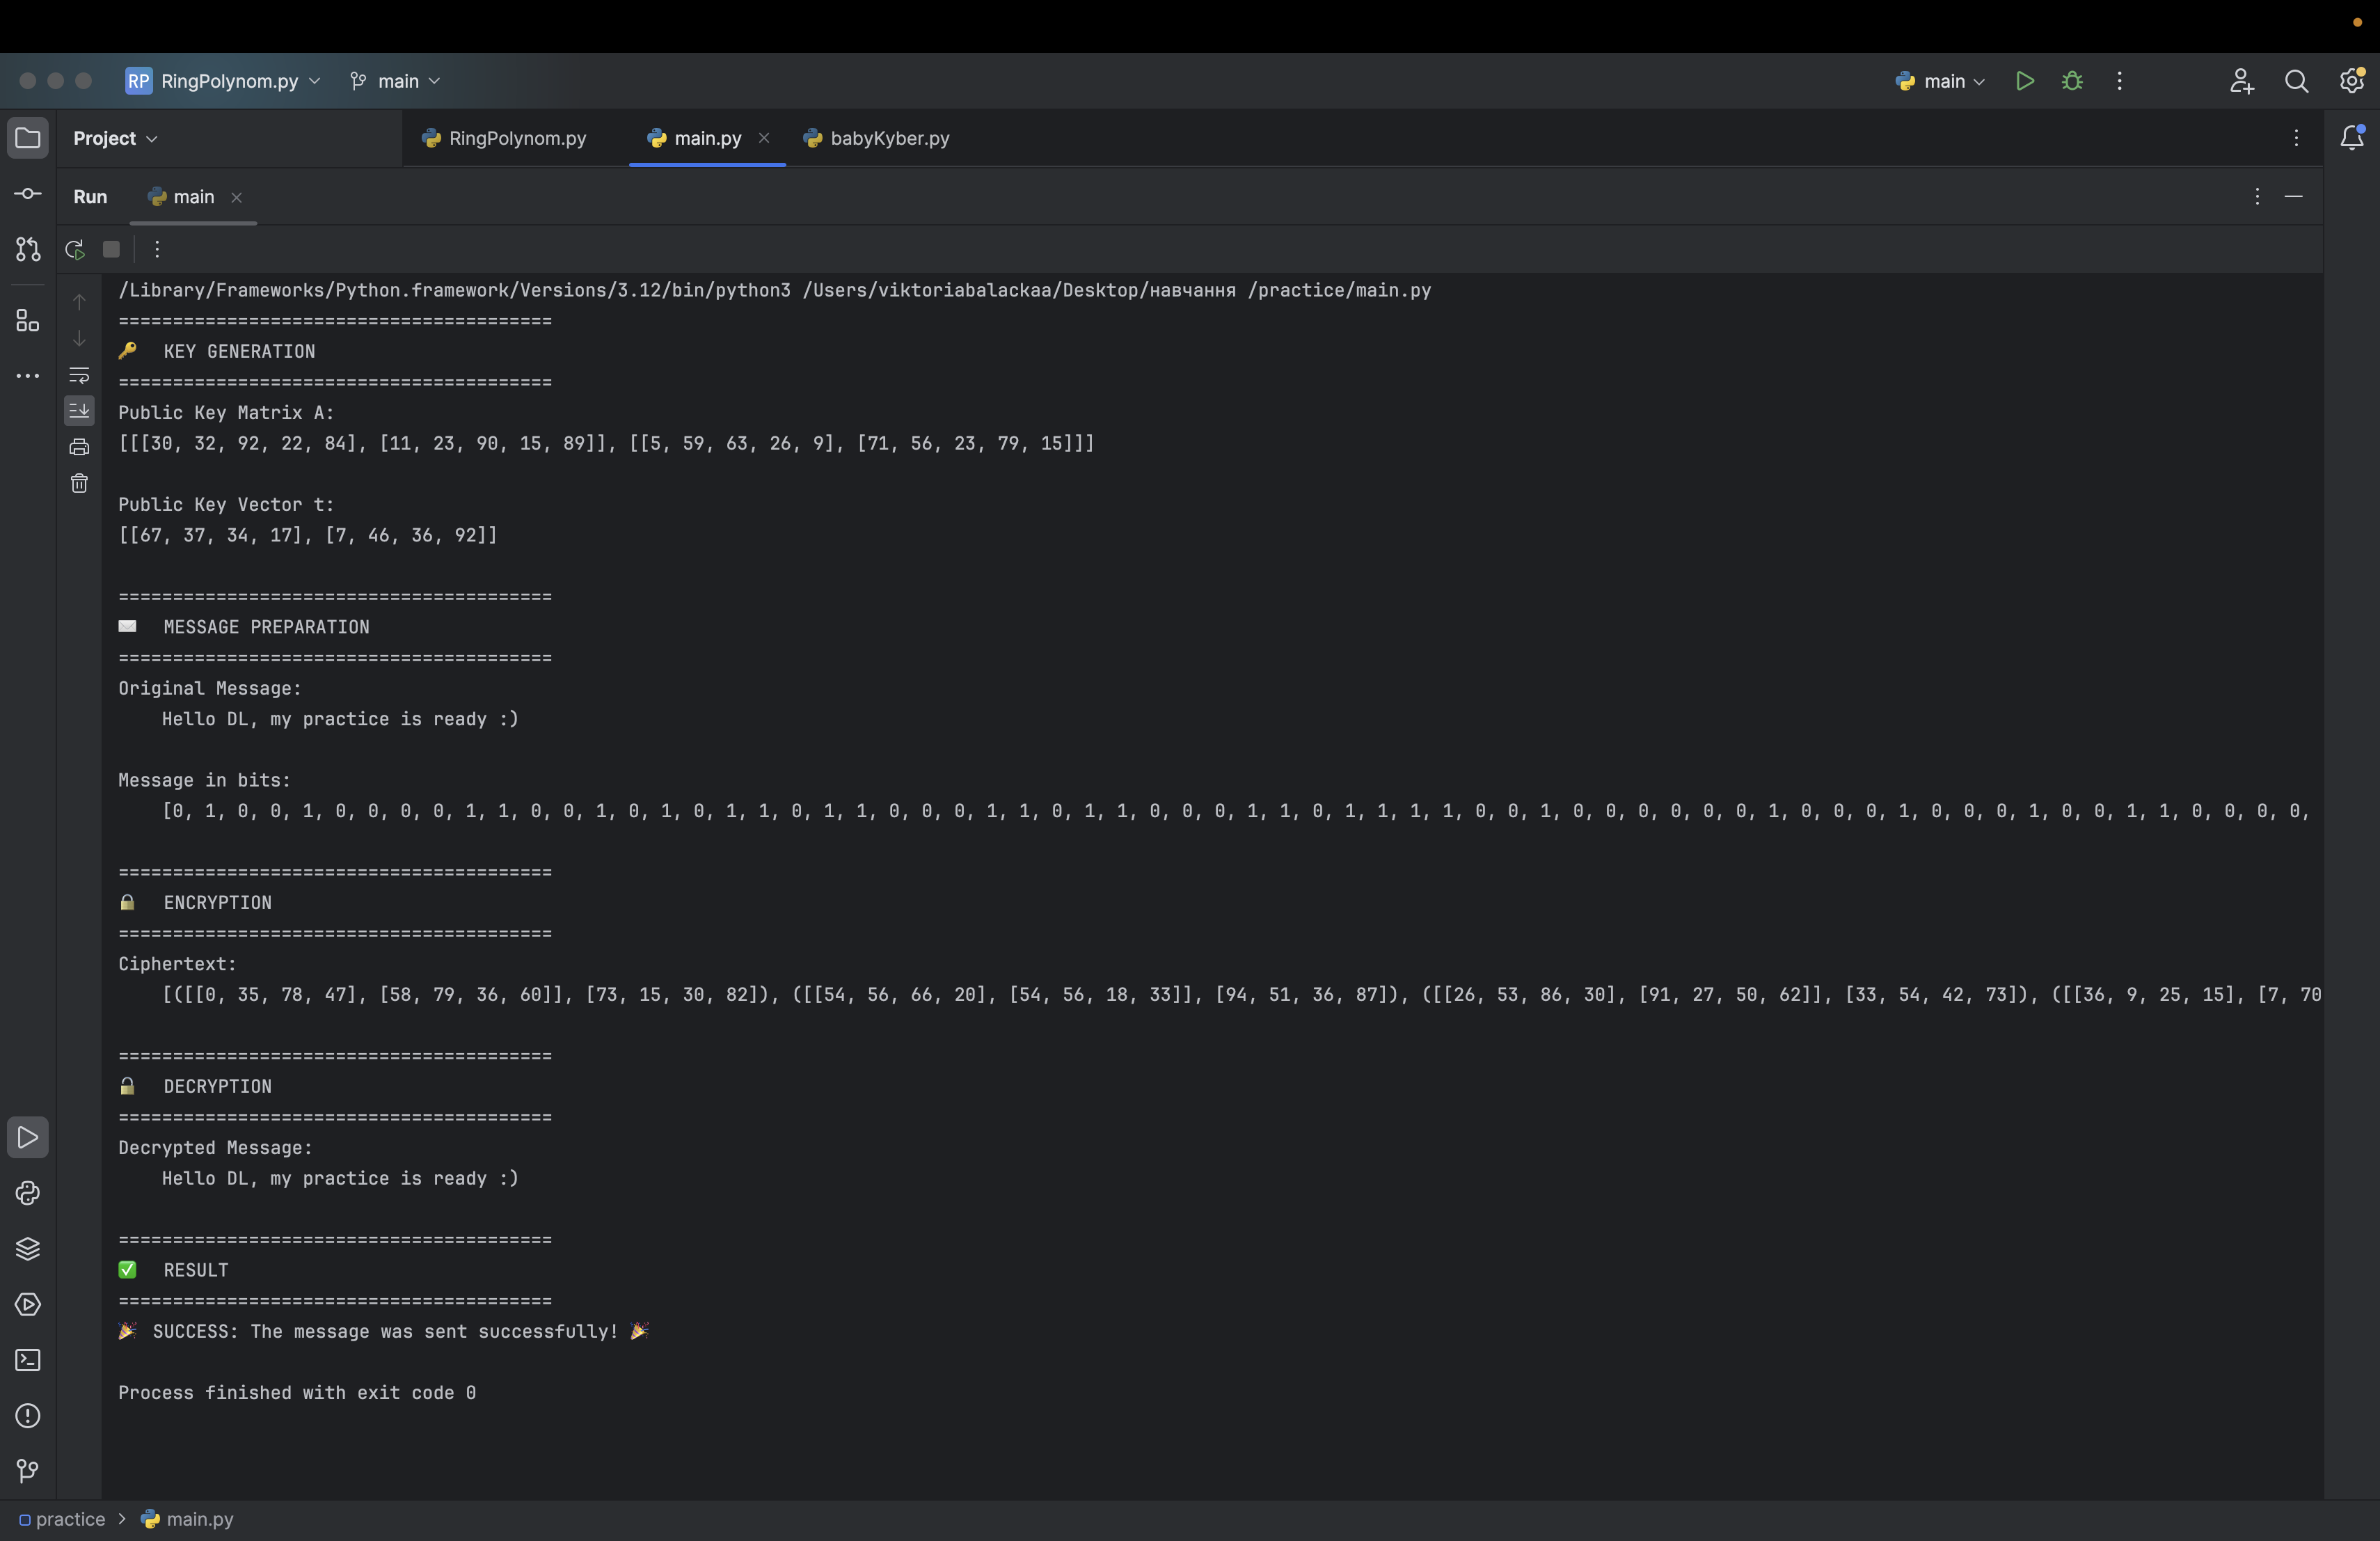
\includegraphics[width=\textwidth]{ПРАКТИКА/Images/test_1.png}
    \caption{Результат 1}
\end{figure}

\begin{figure}[h]
    \centering
    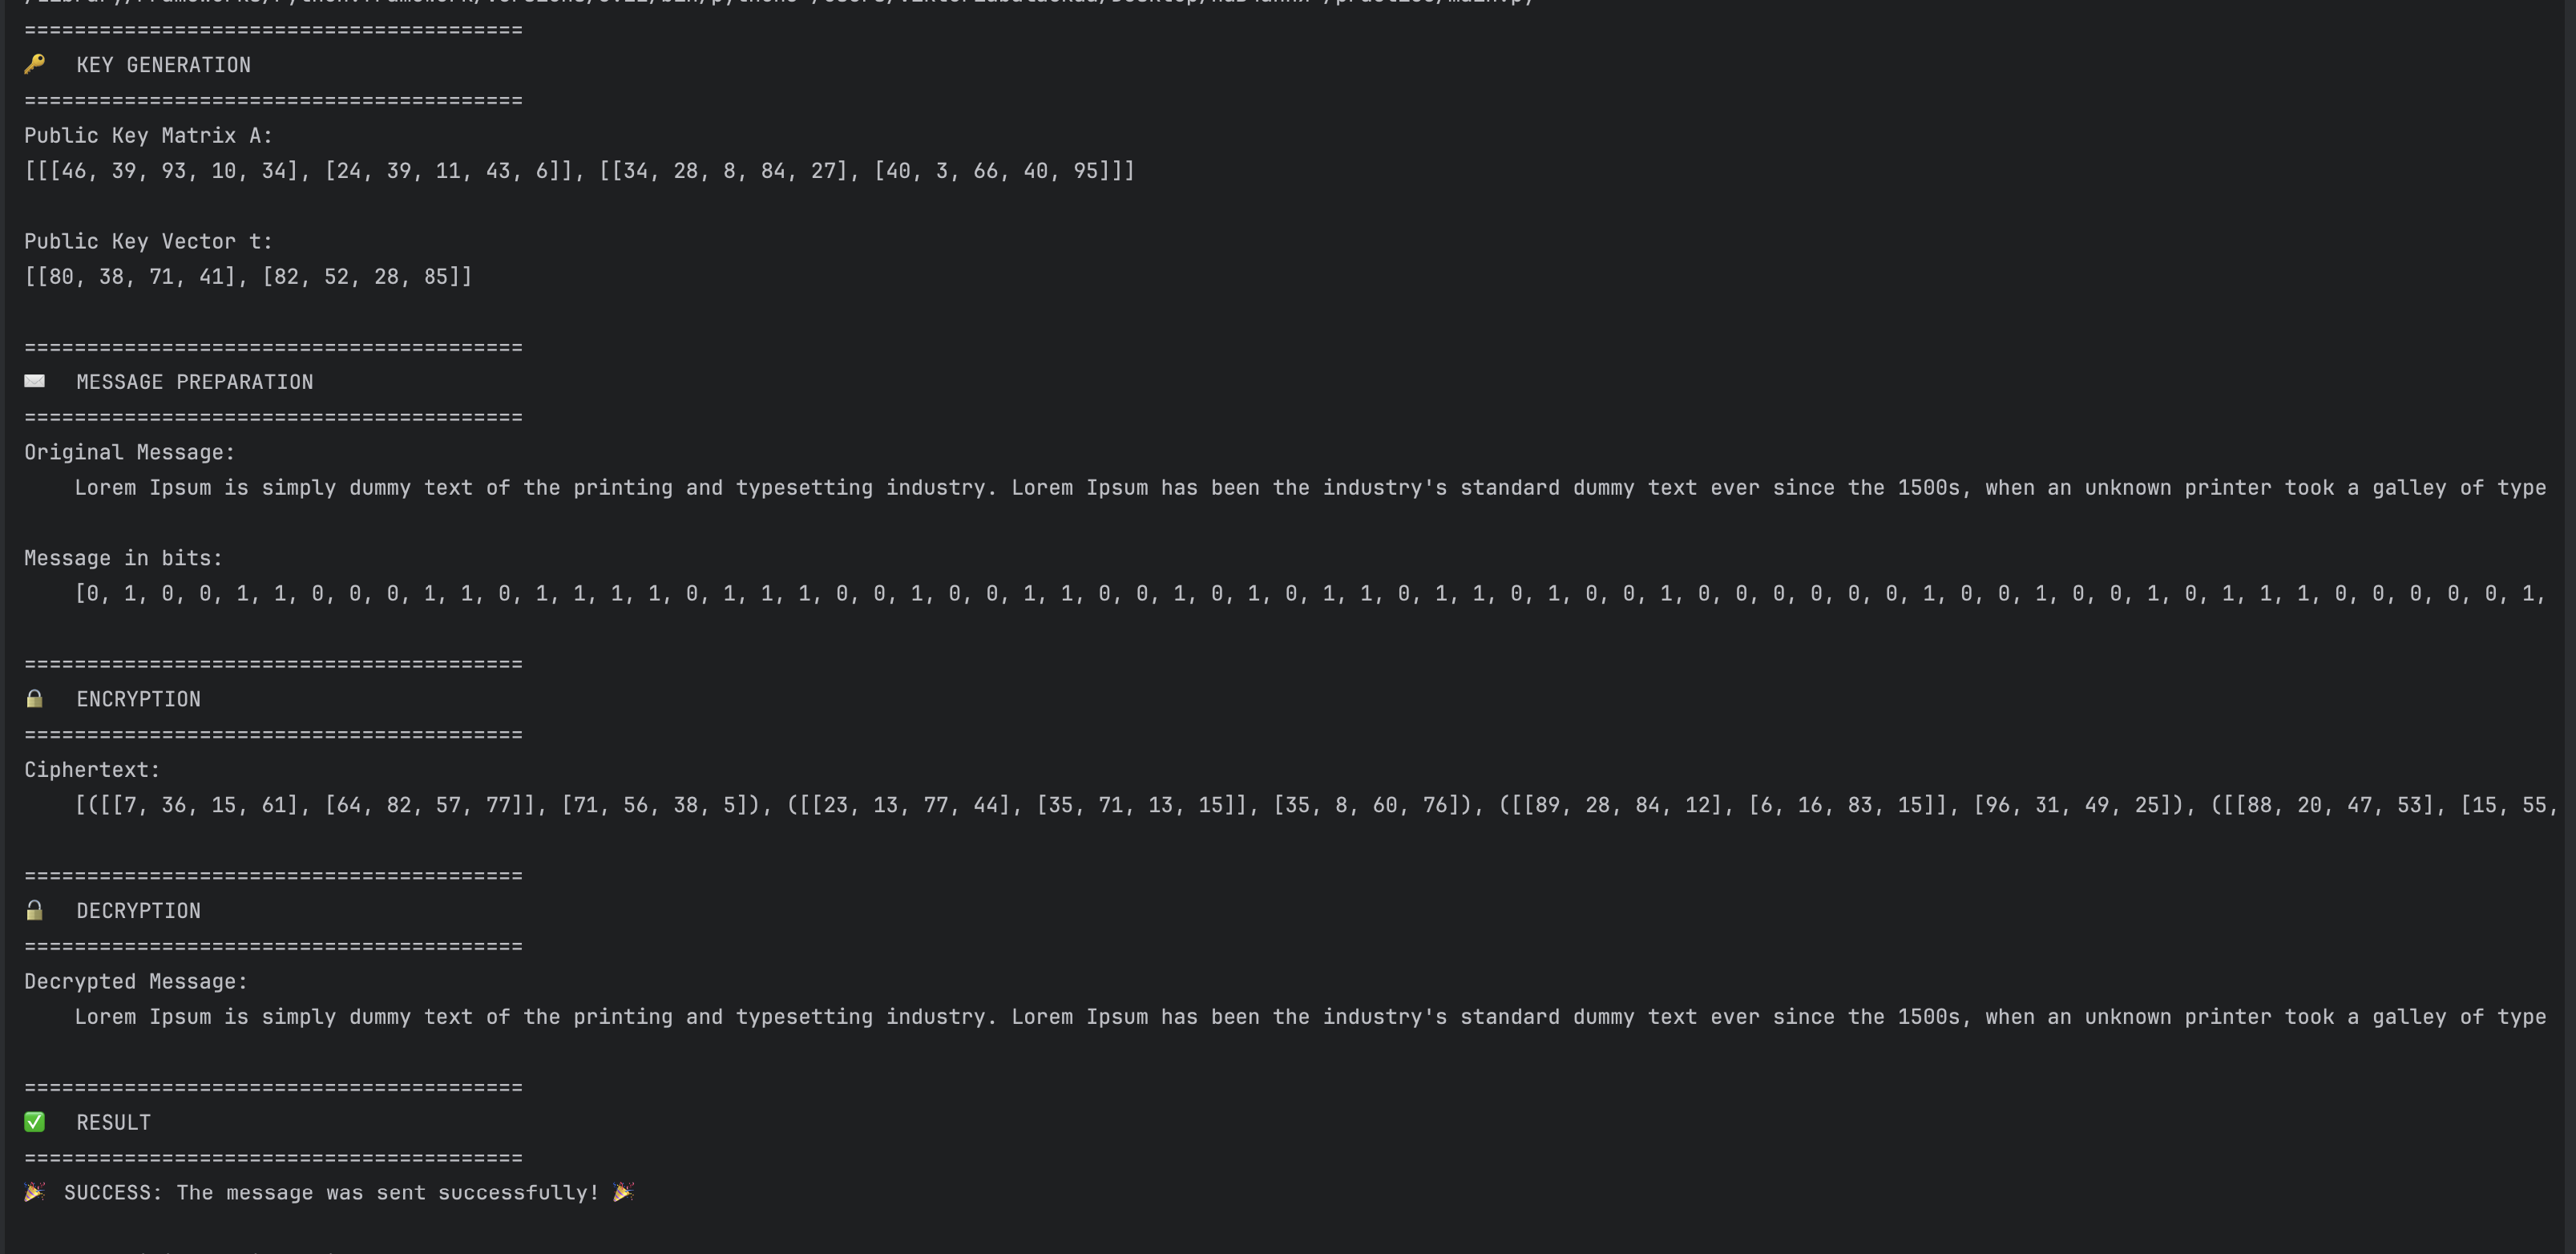
\includegraphics[width=\textwidth]{ПРАКТИКА/Images/test_2.png}
    \caption{Результат 2}
\end{figure}

\begin{figure}[h]
    \centering
    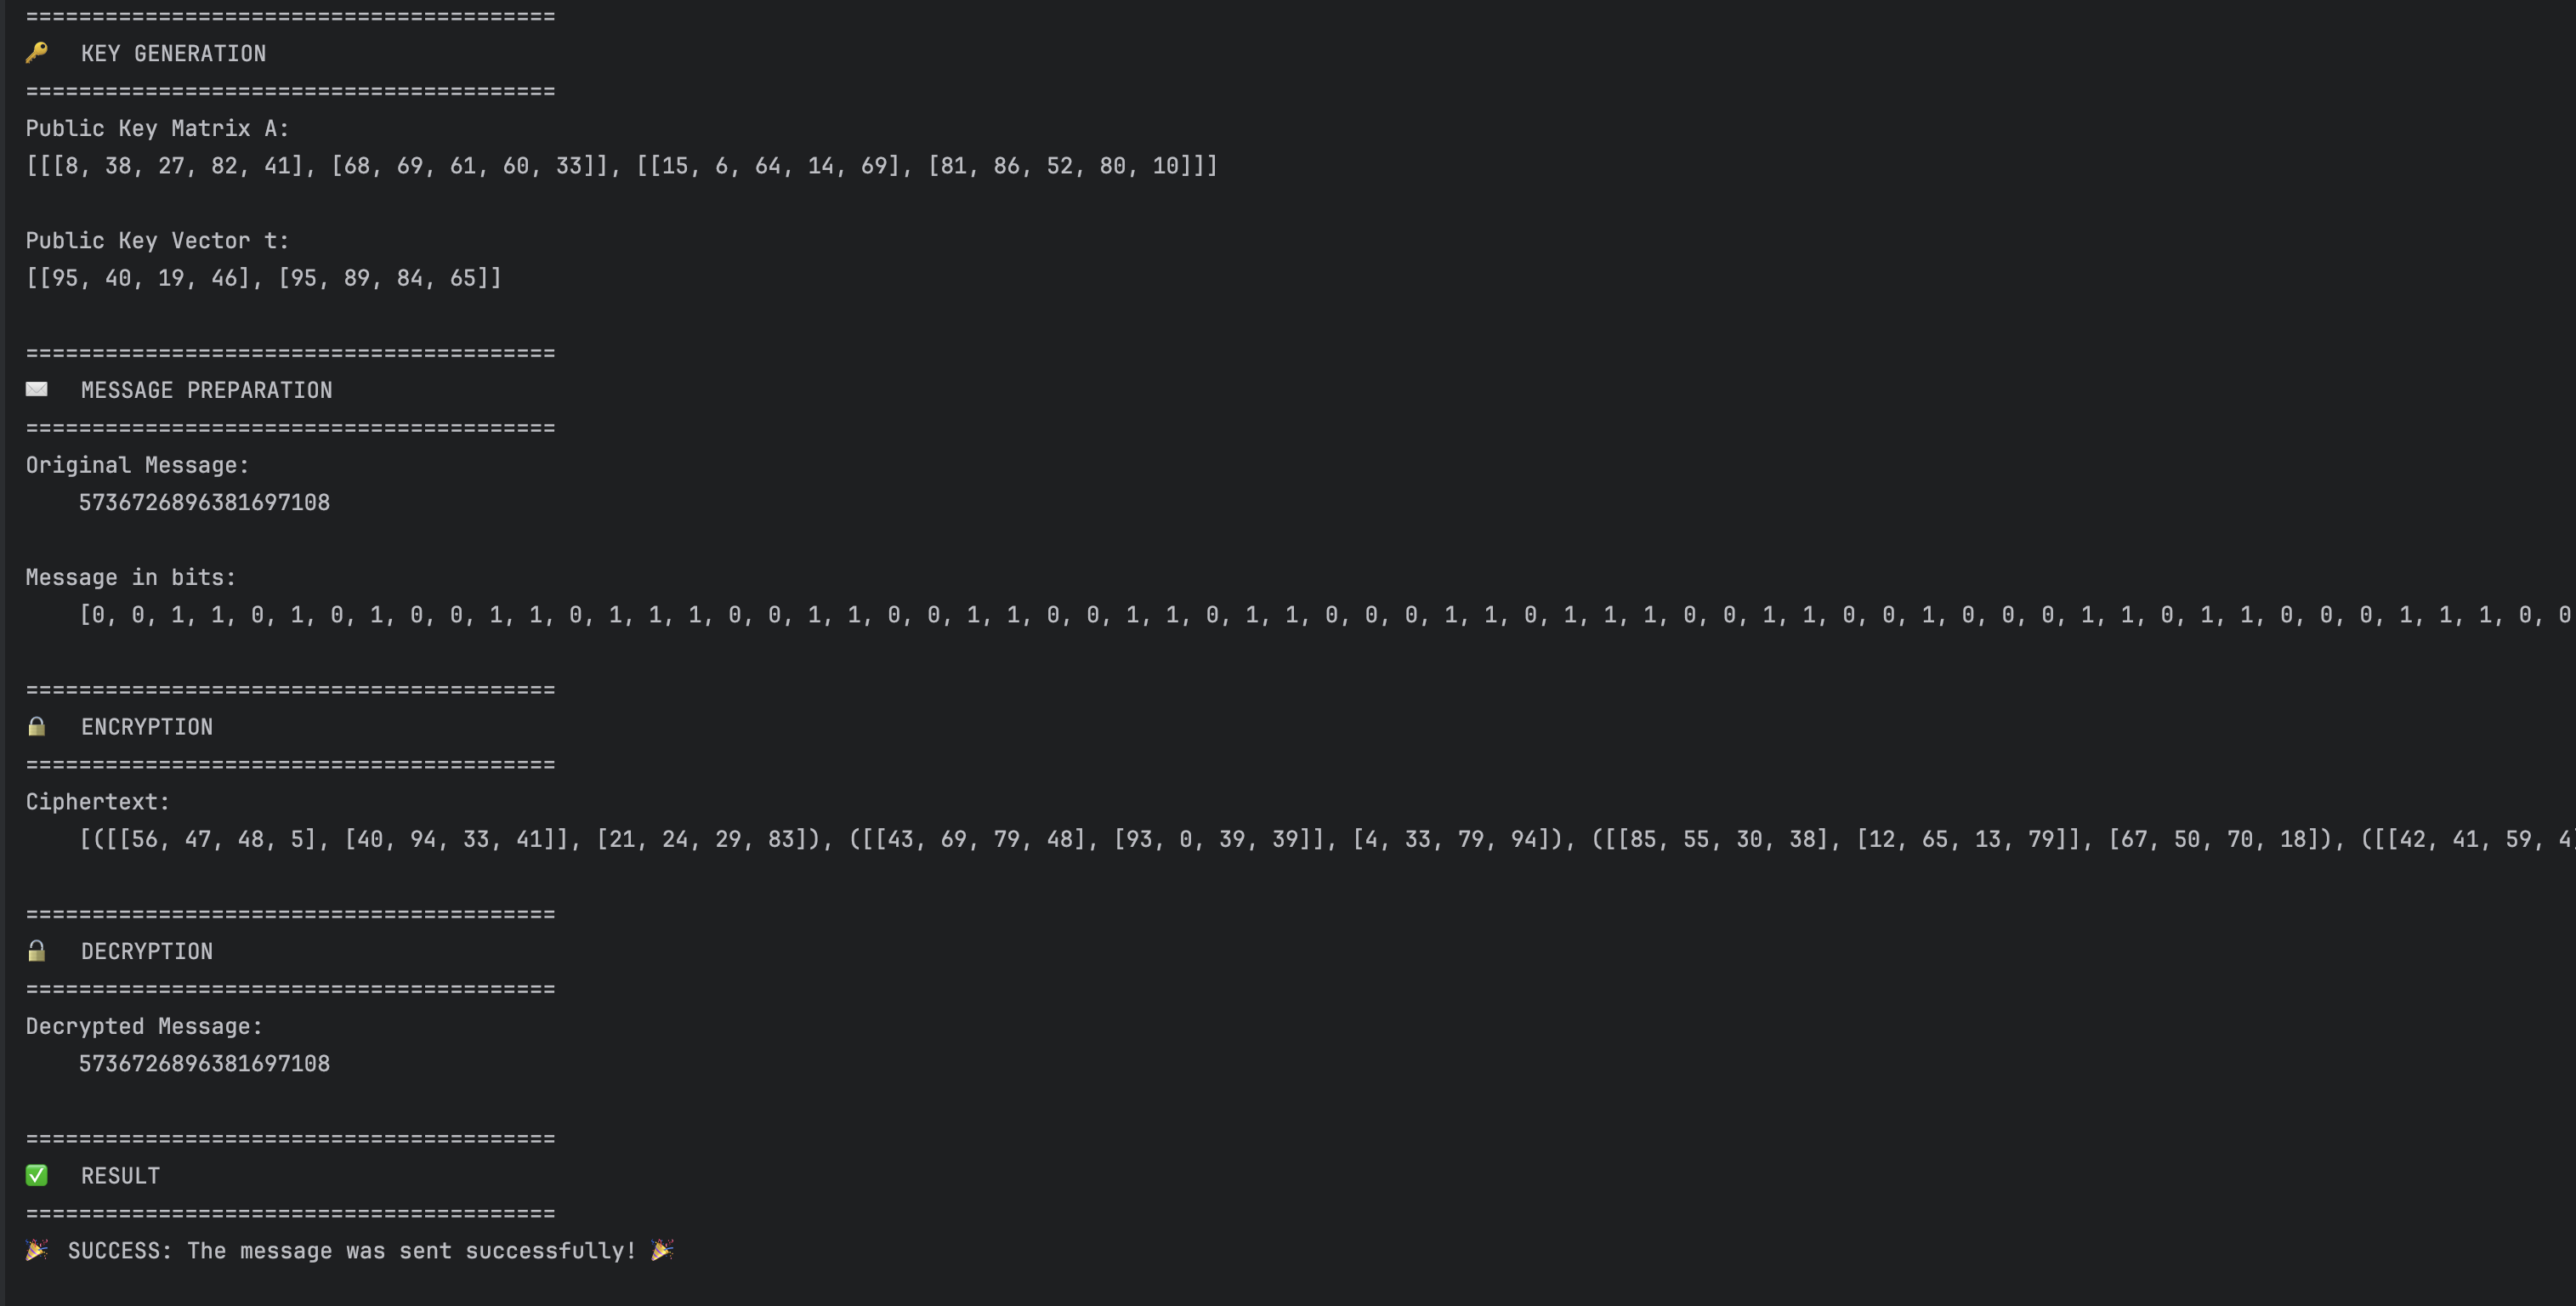
\includegraphics[width=\textwidth]{ПРАКТИКА/Images/test_3.png}
    \caption{Результат 3}
\end{figure}

\begin{figure}[h]
    \centering
    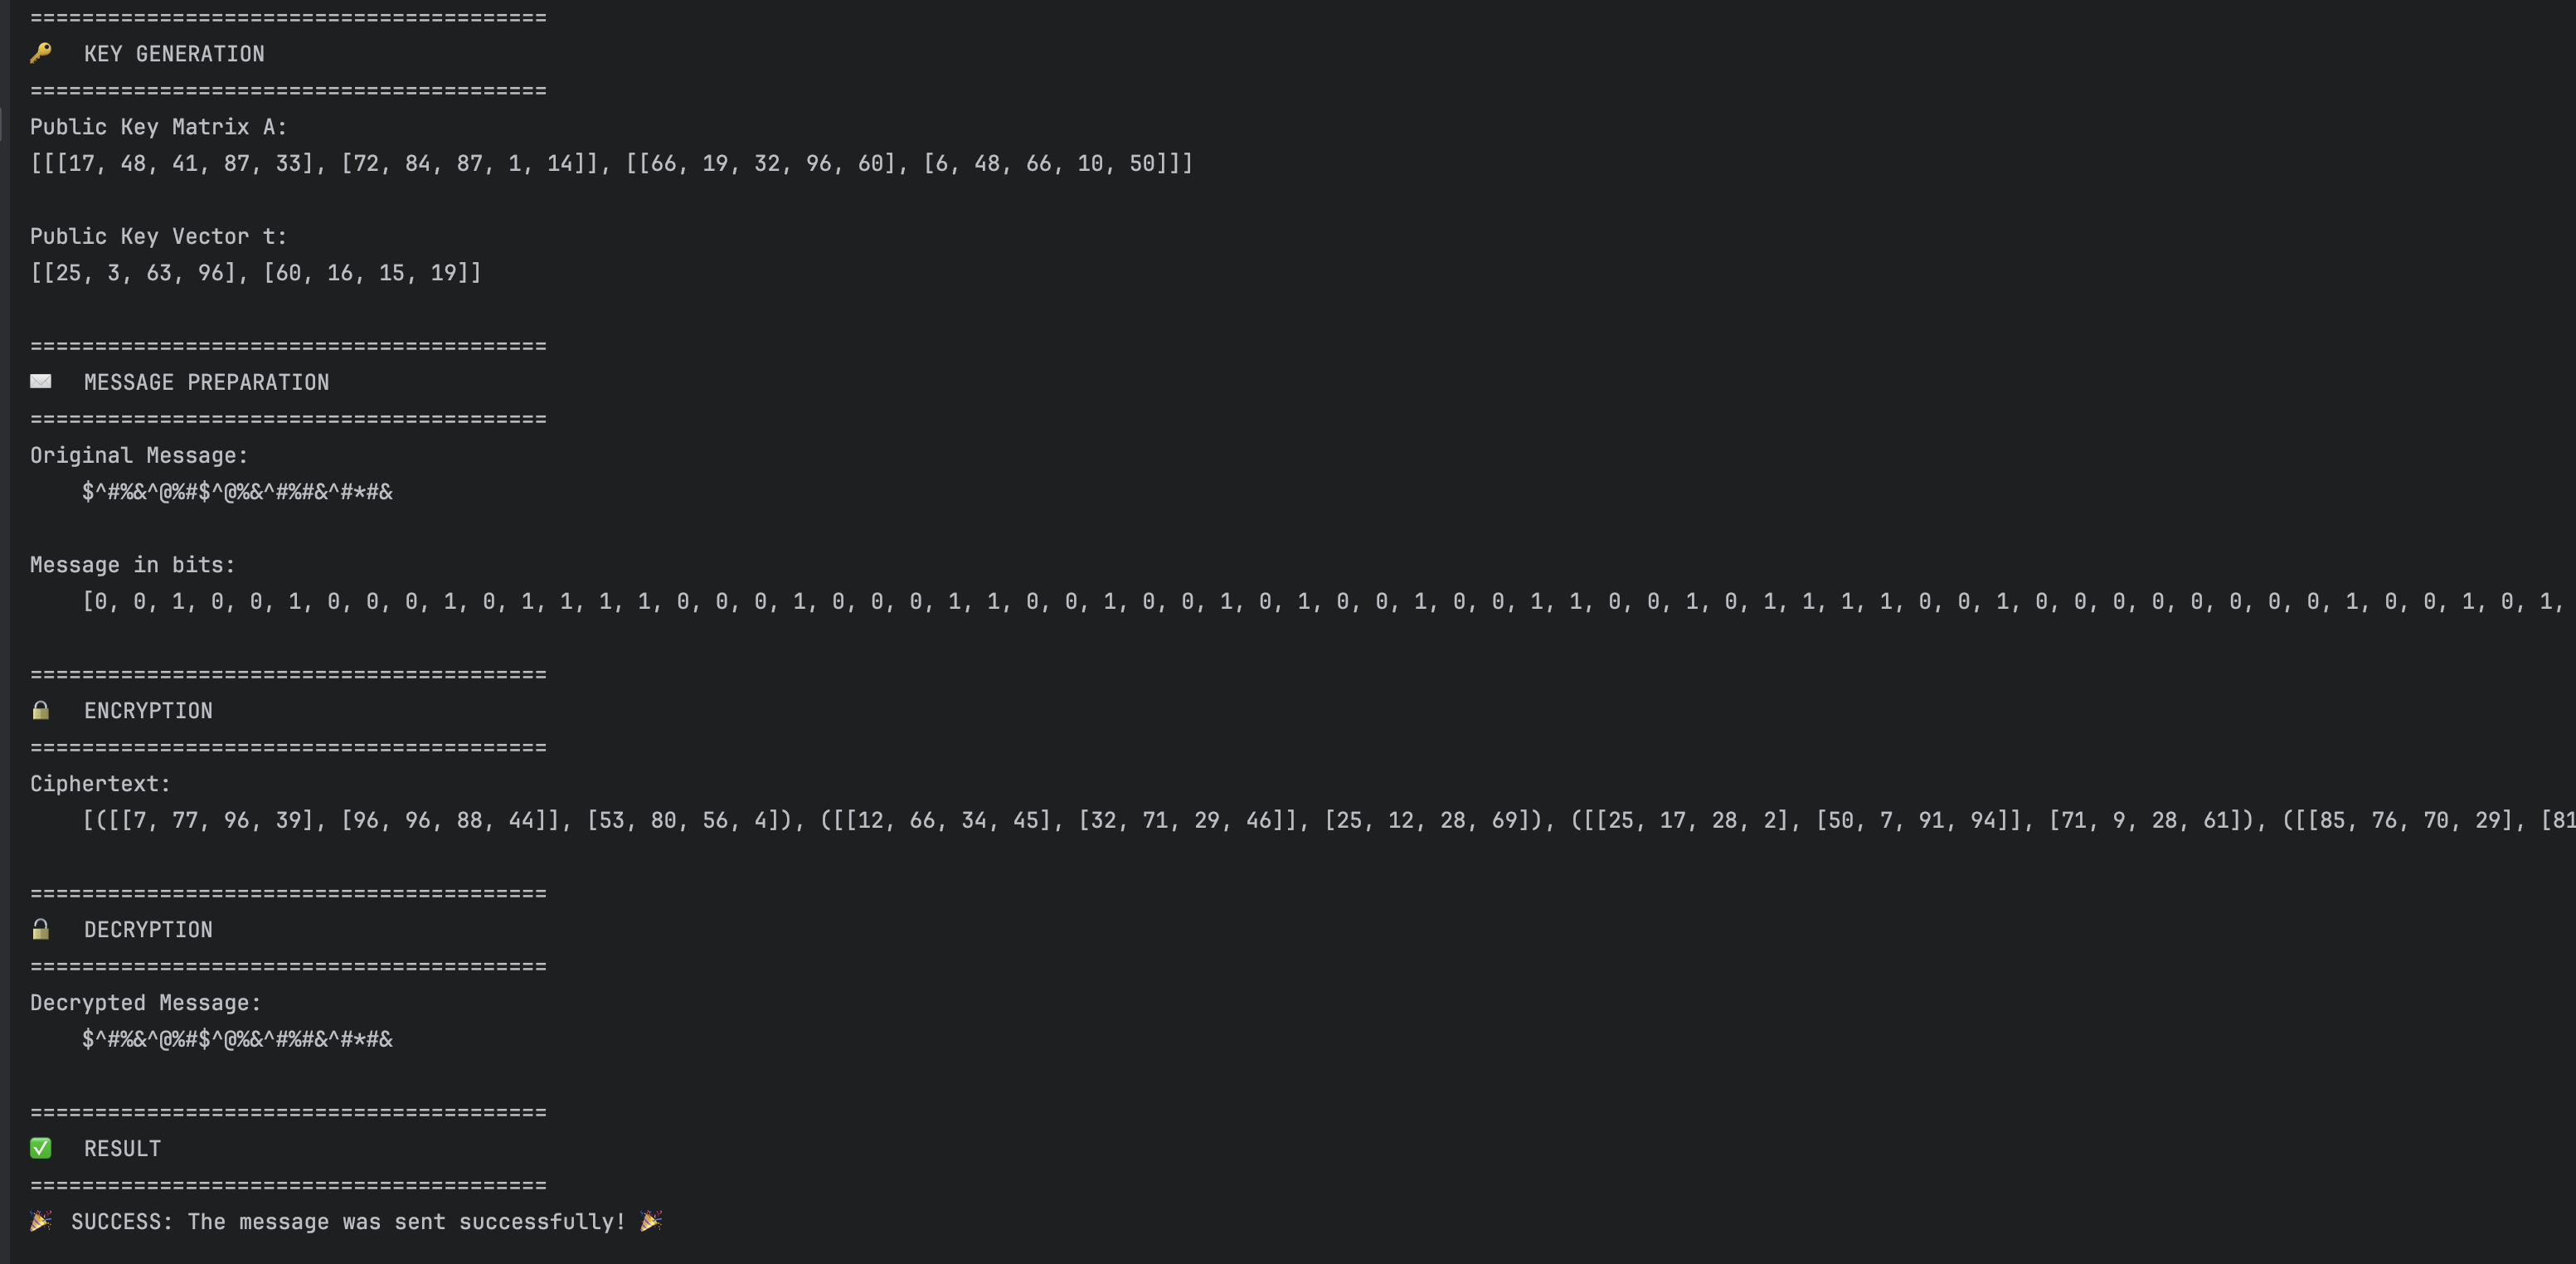
\includegraphics[width=\textwidth]{ПРАКТИКА/Images/test_4.png}
    \caption{Результат 4}
\end{figure}

\begin{figure}[h]
    \centering
    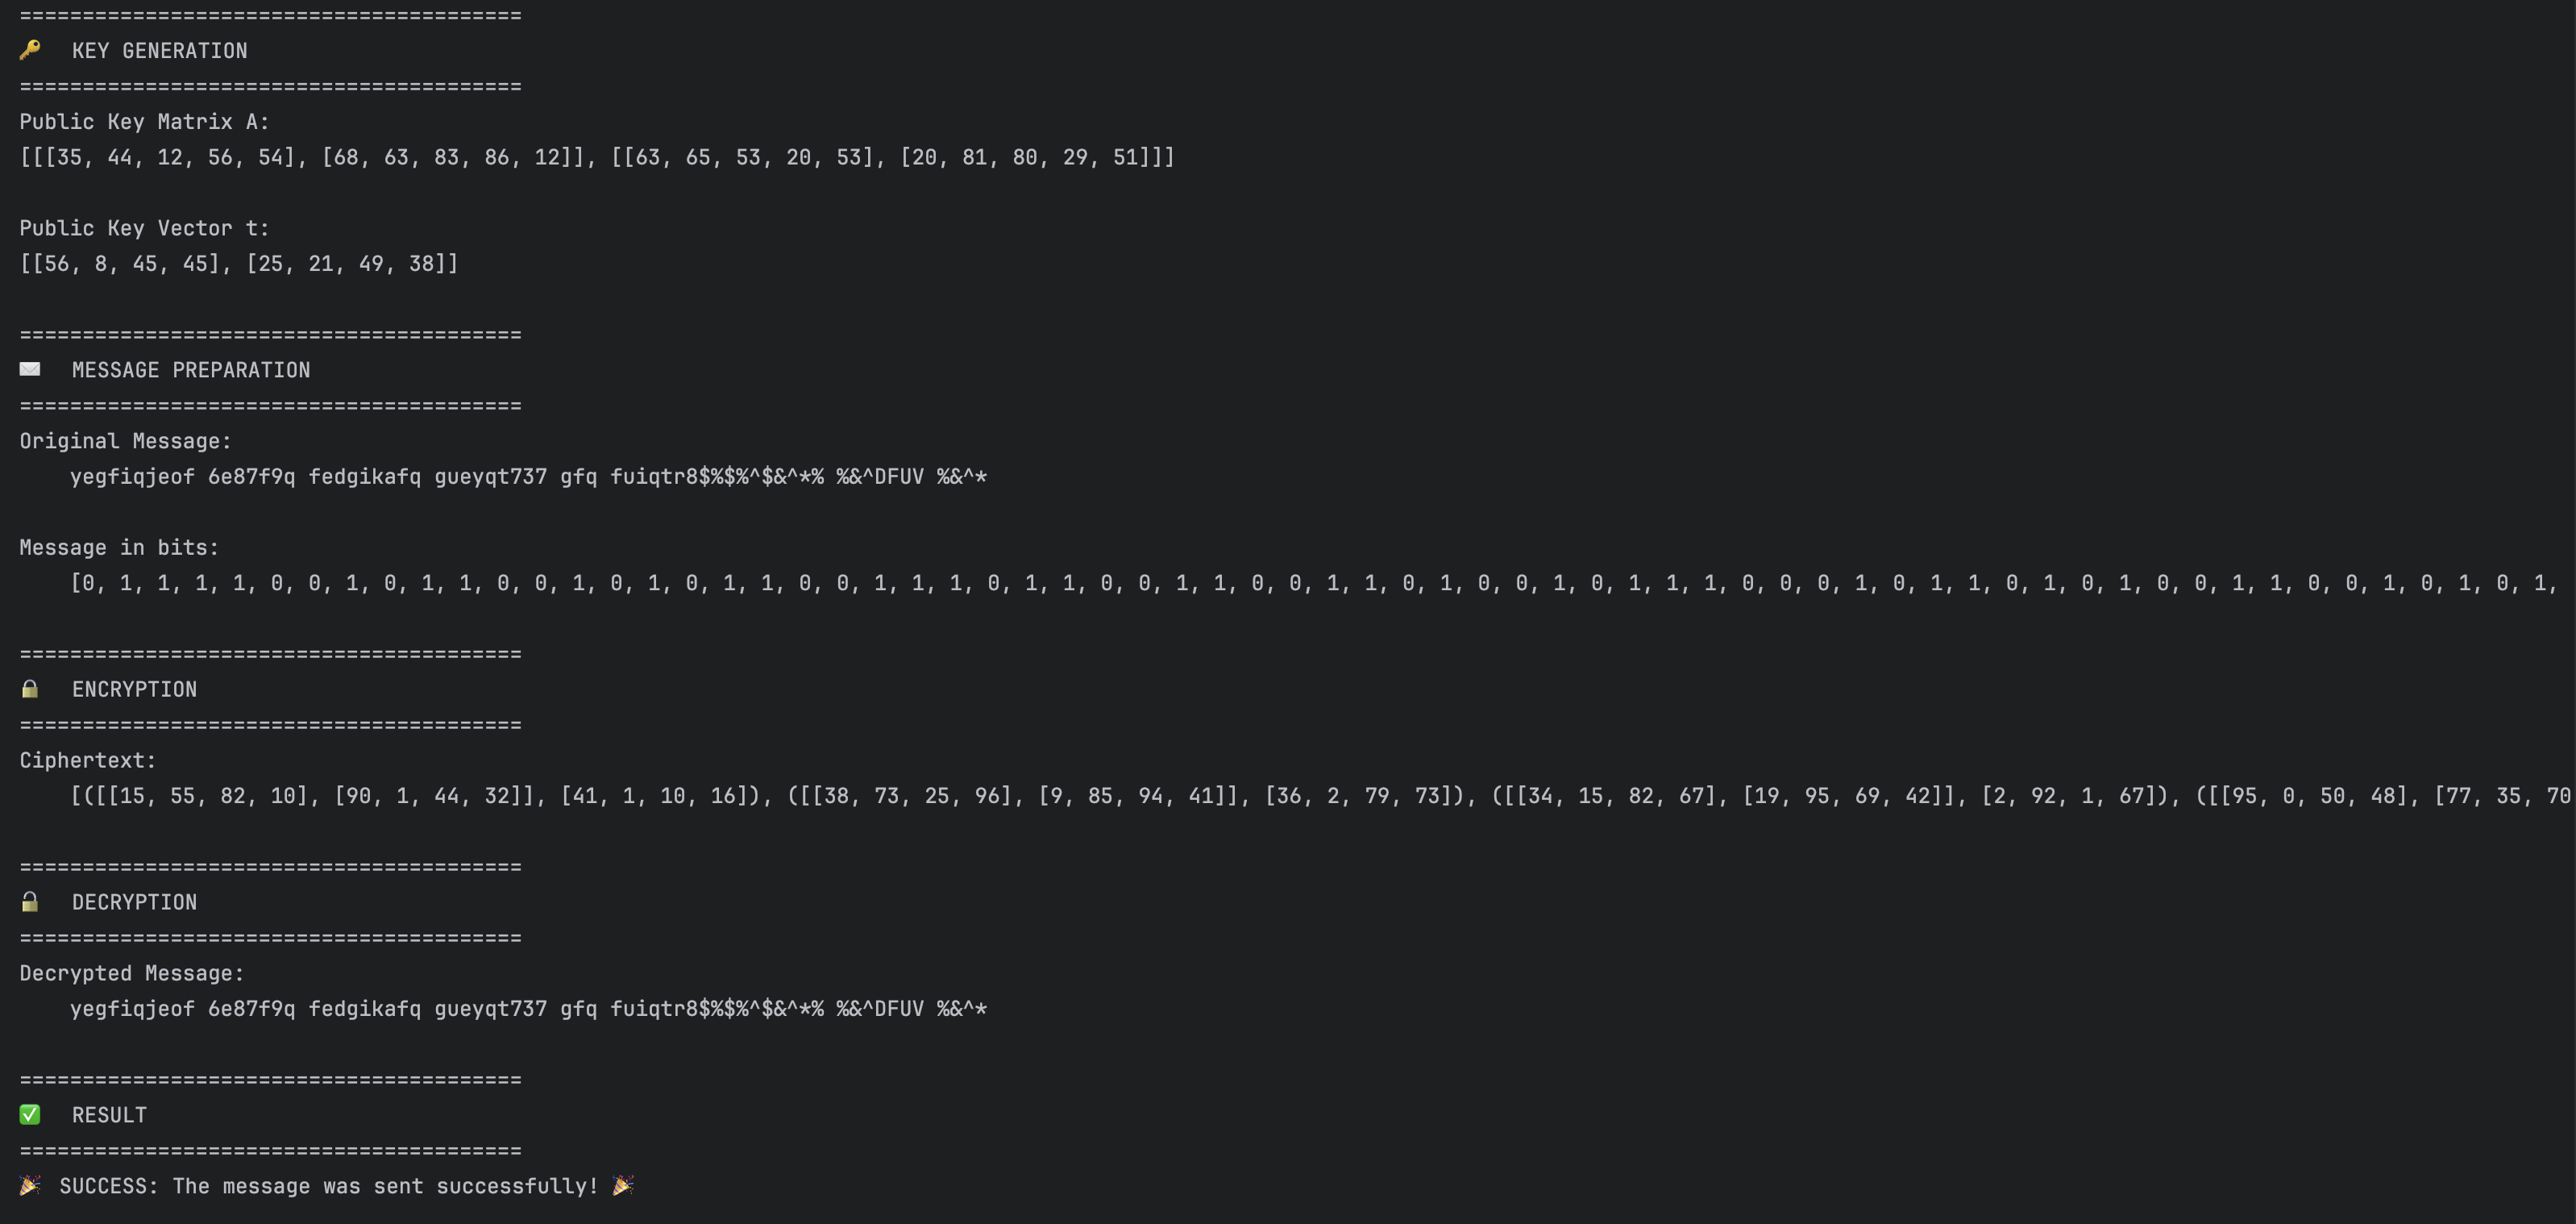
\includegraphics[width=\textwidth]{ПРАКТИКА/Images/test_5.png}
    \caption{Результат 5}
\end{figure}